\documentclass[11pt,twoside,a4paper,listof=totoc]{scrbook}

%Datei f�r die angepassten Styles laden
\usepackage{HTWKstyle}
\usepackage[numbers]{natbib}
\usepackage{latexsym}
%\usepackage{a4wide}
\usepackage{logicdefs}
\usepackage{amssymb}
\usepackage{multicol}
\usepackage{tikz}
\usetikzlibrary{arrows}
\usetikzlibrary{shadows}
\usetikzlibrary{shapes}
\usetikzlibrary{backgrounds}
\usetikzlibrary{positioning}
\tikzstyle{vertex}=[circle,draw,thick,inner sep=3pt,minimum size=6mm]
\tikzstyle{level 1}=[sibling distance=20mm]
\tikzstyle{level 2}=[sibling distance=10mm]
\tikzstyle{level 3}=[sibling distance=5mm]
\tikzstyle{empty}=[sibling distance=5mm]
\tikzstyle{rechteck}=[rectangle,draw,thick,inner sep=4pt]
\tikzset{packet/.style={rectangle, draw, very thick,
minimum size=6mm, rounded corners=1mm}}

\newcolumntype{r}{p{2cm}}

\begin{document}

\begin{titlepage}
\vspace*{-3.5cm} % nach oben verschieben
\enlargethispage{3cm} % unteren Rand verlängern

%_______________LOGO_______________%
 
\begin{flushleft}
\begin{figure} [!htb]
\begin{minipage}{1\textwidth} 
 \vskip 1.0 cm
 \includegraphics[width=4cm]{img/logo.png}% 
\end{minipage} 
\end{figure}
\end{flushleft}

 %____________LOGO_ENDE____________%
  \vspace{-0.7cm}
  \normalsize
  \textsf{Fakult�t Informatik, Mathematik und Naturwissenschaften}
%   \\

\begin{center}
  \vspace{3cm}
  \Large
  \textbf{Verifikation der Tiefensuche mit KIV}
  \\
  \vspace{1.8cm}
  \normalsize eingereicht als
  \\
  \vspace{1.0cm}
  \Large 
  \textsc{Pr�fungsrelevante Studienleistung}
  \\
  \vspace{1.0cm}
  \normalsize im Studiengang Informatik (Master)
  \\ 
  \vspace{1.8cm} von
  \\
  \vspace{1.5cm}
  %\begin{tabular}{l}
        Ricardo Hofmann\\
        Matthias Neubert\\
        Stefan Veit \\
        %\textsf{Studiengang Informatik}
 %\end{tabular}
 
  
  \vspace{2.0cm}
 Leipzig, \today
   \\
  \vspace{3.0cm}
\end{center}
%\begin{flushleft}
 \begin{tabular}{ll}
    Betreuender Professor: & Prof. Dr. Uwe Petermann
 \end{tabular}
  
   
  \vspace{1.5cm}

\end{titlepage}
        % Einf�gen des Titelblatts

\cleardoublepage

\pagenumbering{Roman}       %Seitennummerierung r�misch Gro�buchstaben

\tableofcontents

\pagenumbering{arabic}          %Seitennummerierung Zahlen

\chapter{Einleitung}

%\newpage

\section{Aufgabenstellung}

Innerhalb der Lehrveranstaltung Programmverifikation ist es die Aufgabe, f�r
eine selbstgew�hlte Problemstellung ein Verifikationsprojekt mit Hilfe der
Software \emph{KIV} (Karlsruhe Interactive Verifier) zu erstellen. F�r die
vorliegende Arbeit wurde diesbez�glich das Problem der Tiefensuche auf Graphen
betrachtet. Dabei handelt es sich um einen Algorithmus, der mittels der
Strategie der \glqq{}Tiefen-Zuerst-Suche\grqq{} die Existenz von Pfaden - von
einem gegebenen Startknoten zu einer Zielknotenmenge - pr�ft respektive in
einer modifizierten Variante den dabei resultierenden Pfad zur�ckgibt. 
\par
Eine genaue Beschreibung des Algorithmus sowie der �berblick �ber die konkrete
Umsetzung des Projektes wird Gegenstand der folgenden Kapitel sein.

\section{Motivation}

Die Graphentheorie ist ein wichtiges Gebiet innerhalb der Informatik. F�r
viele Problemstellungen dient die Datenstruktur Graph der Abstraktion und
Abbildung verschiedenster Fragestellungen.
\par
Speziell f�r das Verifikationswerkzeug KIV fehlen jedoch diesbez�glich
noch entsprechende Bibliotheken. Ein erster Ansatz wurde durch die
Umsetzung der Graphenbibliothek durch das studentische Projekt von Marc Drobek
und David Redlich realisiert. Aufbauend auf dieser bereits vorhandenen
Spezifikation/Implementierung soll dieses Projekt die Bibliothek um die
algorithmische Herangehensweise der sogenannten Tiefensuche anreichern. Die im
Weiteren beschriebenen Umsetzungen und Ma�nahmen zur Spezifikation,
Implementierung bis hin zur Verifikation sollen dies veranschaulichen.


\section{Gliederung der Arbeit}

Die folgenden Kapitel besch�ftigen sich mit der konkreten Beschreibung der
betrachteten Problemstellung sowie der Erl�uterung der eingef�hrten
Spezifikationen.
\par
Kapitel \ref{chap:problembeschreibung} wird dabei insbesondere auf die Tiefensuche, deren
Implementierung sowie die Umsetzung in KIV eingehen.
\par
Ein detaillierteren Einblick in die Realisierung innerhalb des Karlsruhe
Interactive Verifiers bietet Kapitel \ref{chap:spezifikation}, welches auf die einzelnen
Spezifikationen, die implementierten Module sowie verwendete Hilfss�tze
eingeht.
\par
Den Abschluss wird Kapitel \ref{chap:zusammenfassung} bilden, wo die wichtigsten Kernpunkte der
Arbeit nochmals zusammengefasst sind.

     

\chapter{Problembeschreibung}

%\newpage

\section{Tiefensuche}
\label{sec:tiefensuche}

Die Tiefensuche ist ein Verfahren zum Traversieren von Graphen. Das Ziel besteht darin einen Knoten zu finden, der zu einer gegebenen Zielknotenmenge geh�rt. Die Suche ist genau dann erfolgreich, wenn ein Pfad von einem gegebenen Startknoten zu einem Zielknoten aus der Zielknotenmenge existiert.
\par
Es werden zun�chst vom Startknoten alle direkt erreichbaren Knoten ermittelt, d.h. Knoten, die durch eine Kante mit dem Startknoten verbunden sind. Diese Knoten werden in eine open-Liste eingetragen. Auf der open-Liste befinden sich alle Knoten, die von einem expandierten Knoten erreichbar sind, selbst aber noch nicht expandiert wurden. Unter "`expandieren"' ist das Ermitteln der Nachbarknoten zu verstehen. Knoten, die bereits expandiert wurden, werden in die close-Liste eingetragen, um sie nicht nochmals zu untersuchen. Bei der Expansion eines Knotens werden nur Knoten ber�cksichtigt, die sich noch nicht auf der close-Liste befinden. Alle entdeckten Nachfolgerknoten werden vorn an die open-Liste angehangen. Daher kann die open-Liste als Stack betrachtet werden (LIFO-Prinzip). Durch die Verwendung dieser Datenstruktur unterscheidet sich die Tiefen- von der Breitensuche.
\par
Von der open-Liste wird nun immer der erste Knoten entnommen, auf die close-Liste gesetzt und expandiert. Die erhaltenen Nachfolgerknoten werden jeweils der open-Liste hinzugef�gt.
\par
Die Suche endet, sobald ein Knoten aus der Zielknotenmenge erreicht wurde oder die open-Liste leer ist. Im letztgenannten Fall existiert kein Pfad vom Startknoten zu einem Zielknoten.
\par
Die Funktionsweise wird anhand des in Abb. \ref{fig:dfs-ex} gezeigten Beispielgraphen verdeutlicht. Dabei ist a der Startknoten und e der einzige Knoten in der Zielknotenmenge. In Tabelle \ref{tab:dfs-ex} sind alle Bearbeitungsschritte der Tiefensuche aufgef�hrt. Es wird jeweils angegeben, welcher Knoten bearbeitet wird und welche Elemente sich nach der Bearbeitung dieses Knotens auf der open- und close-Liste befinden.

\begin{figure}[!h]
\centering
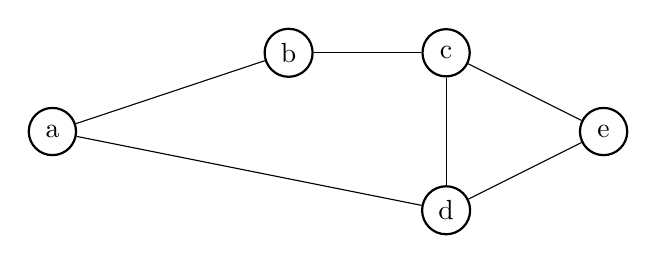
\begin{tikzpicture}
	\node[vertex] (1) at (1,0) {a};
	\node[vertex] (2) at (4,1) {b};
	\node[vertex] (3) at (6,-1) {d};
	\node[vertex] (4) at (6,1) {c};
	\node[vertex] (5) at (8,0) {e};
	%\node (3) at (4,0) {...};
	\path [-] (1) edge node [above] {} (2);
	\path [-] (1) edge node [above] {} (3);
	\path [-] (2) edge node [above] {} (4);
	\path [-] (3) edge node [above] {} (4);
	\path [-] (3) edge node [above] {} (5);
	\path [-] (4) edge node [above] {} (5);	
\end{tikzpicture}
\caption{Beispielgraph}
\label{fig:dfs-ex}
\end{figure}

\begin{table}[!htp]
\begin{center}
\begin{tabular}{c|p{2cm}|p{2cm}}
  %\hline
  bearb. Knoten & open & close \\
  \hline
  Init. & [a] & [] \\
  a & [b, d] & [a] \\
  b & [c, d] & [a, b] \\
  c & [e, d] & [a, b, c] \\
  e & \multicolumn{2}{c}{Abbruch mit R�ckgabewert \texttt{true}} \\
	\end{tabular}
	\caption{Abarbeitungschritte f�r Beispielgraphen}%
	\label{tab:dfs-ex}%
	\end{center}
\end{table}
\section{Implementierungen}
\label{sec:implementierungen}

\par
\vspace{0.2cm}
\textbf{Rekursive Implementierung}
\par

Die Tiefensuche kann rekursiv wie in Listing \ref{lst:dfs-rek} als Pseudocode dargestellt implementiert werden. Die Funktion wird mit den Paramentern \texttt{open = Startknoten}, \texttt{close = leere Liste}, \texttt{ziel = Zielknotenmenge} und \texttt{graph = zu untersuchender Graph} aufgerufen.
\par
Zu Beginn wird gepr�ft, ob sich der aktuell betrachtete Knoten in der Zielknoten befindet. Ist dies der Fall wird \texttt{true} als Ergebnis zur�ckgegeben. Ansonsten wird der Knoten der close-Liste hinzugef�gt und expandiert. Auf die Implementierung der Funktion \texttt{expand} wird nicht n�her eingegangen. Sie bestimmt die Nachbarn eines Knotens unter Ausschluss derjenigen, die sich bereits auf der close-Liste befinden.
\par
Ist die open-Liste nach diesem Bearbeitungsschritt nicht leer, so erfolgt ein rekursiver Aufruf der Funktion.

\begin{figure}[!h]
\begin{lstlisting}[caption=Pseudocode rekursive Tiefensuche, label=lst:dfs-rek]
dfs-rek(open, close, ziel, graph)
{
  knoten = open.pop;
  if (knoten in ziel)
  {
    return true;
  }
  else
  {
    close := knoten + close;
    open := expand (knoten, close) + open;
    
    if(open.isEmpty == false)
    {
      dfs-rek(open, close, ziel, graph);
    }
    else
    {
    	return false;
    }
  }
}

\end{lstlisting}
\end{figure}

\par
\vspace{0.2cm}
\textbf{Iterative Implementierung}
\par

Eine iterative Variante der Tiefensuche ist in Listing \ref{lst:dfs-it} als Pseudocode dargestellt. Die Aufrufparameter der Funktion sind der Startknoten (\texttt{startknoten}), die Zielknotenmenge (\texttt{ziel}) und der zu untersuchende Graph (\texttt{graph}). 
\par
Nach der Initialisierung der open- und close-Liste wird eine while-Schleife solange durchlaufen, bis die open-Liste leer ist oder vorzeitig mit der R�ckgabe von \texttt{true} abgebrochen wird. In der Schleife wird der erste Knoten der open-Liste entnommen und gepr�ft, ob dieser zur Zielknotenmenge geh�rt. Ist dies der Fall war die Suche erfolgreich und es wird abgebrochen. Andernfalls wird der Knoten der close-Liste hinzugef�gt und expandiert.
\par
Ist die open-Liste nach diesem Schritt leer, wird die Schleife verlassen und \texttt{false} zur�ckgegeben, da die Suche erfolglos war. Ansonsten erfolgt der n�chste Schleifendurchlauf.

\begin{figure}[!h]
\begin{lstlisting}[caption=Pseudocode iterative Tiefensuche, label=lst:dfs-it]
dfs-it(startknoten, ziel, graph)
{
  open := startknoten;
  close := [];
  while(open != empty)
  {
    knoten := open.pop;
    if(knoten in ziel)
    {
      return true;
    }
    else
    {
      close := knoten + close;
      open := expand(knoten, close) + open;
    }  
  }
  return false;
}
\end{lstlisting}
\end{figure}
\section{Umsetzung in KIV}

F�r die Umsetzung und Verifikation der Tiefensuche im KIV wurde die Graphenbibliothek von M. Drobek und D. Redlich verwendet (vgl. \cite{dr:2008}). Darauf aufbauend wurden zwei Spezifikationen entwickelt.
\par
\texttt{digraph-dfs-proc} spezifiziert die Tiefensuche, wie in Abschnitt \ref{sec:tiefensuche} beschrieben. Das bedeutet der R�ckgabewert ist entweder \texttt{true} oder \texttt{false}, abh�ngig davon, ob ein Knoten aus der Zielknotenmenge erreicht werden kann oder nicht. Eine genauere Beschreibung der Spezifikation erfolgt im Abschnitt \ref{sec:digraph-dfs-proc}.
\par
Dieser Spezifikation gen�gen die Module \texttt{dfs-it-1} als iterative Implementierung sowie \texttt{dfs-rek-1} als rekursive Implementierung. Details zu diesen Modulen k�nnen den Abschnitten \ref{sec:dfs-it-1} bzw. \ref{sec:dfs-rek-1} entnommen werden.
\par
Die zweite Spezifikation (\texttt{digraph-dfs-func}, vgl. Abs. \ref{sec:digraph-dfs-func}) definiert das Verhalten einer Variante der Tiefensuche, die zus�tzlich den Pfad vom Startknoten zu einem gefundenen Knoten aus der Zielknotenmenge liefert, sofern dieser existiert. F�r diese Spezifikation wurden ebenfalls eine rekursive (\texttt{dfs-rek-func}) und eine iterative Implementierung (\texttt{dfs-it-func-1}) umgesetzt. Genauere Beschreibungen zu diesen Modulen sind in den Abschnitten \ref{sec:dfs-rek-func} und \ref{sec:dfs-it-func-1} zu finden.
\par
Zus�tzlich wurde die Spezifikation \texttt{digraph-path} mit der zugeh�rigen Implementierung \texttt{dfs-temp} erstellt. Diese stellt einen Hilfssatz dar, der die Anzahl der erreichbaren Knoten von einem gegebenen Knoten (z.B. dem Startknoten) spezifiziert. Damit konnte eine Vereinfachung der Terminationsbeweise in den Modulen der Tiefensuche erreicht werden. Details dazu werden im Abschnitt \ref{sec:digraph-path} erl�utert.
\par
Zusammenfassend ist der komplette Projektgraph in Abb. \ref{fig:graph} dargestellt.

\begin{figure}[!htp]
	\centering
		\includegraphics[height=0.7\paperheight]{img/graph.png}
	\caption{Projektgraph KIV}
	\label{fig:graph}
\end{figure}


\chapter{Spezifikation und Module}

%\newpage

\subsection{Spezifikation \texttt{digraph-dfs-proc}}
\label{sec:digraph-dfs-proc}

Ausgehend von den �berlegungen in Kapitel 2 soll zun�chst eine Tiefensuche als Prozedur umgesetzt werden.
Dies bedeutet, dass die R�ckgabe des Programmes ein Wahrheitswert ist. Enth�lt der Pfad G einen Weg zum Startknoten zur Zielknotenmenge, so
wird TRUE zur�ck geliefert, anderfalls FALSE. Im folgenden Absatz sieht man die Signatur der Spezifikation:

digraph-dfs-proc = \\
{\bf enrich} digraph-basic, union\_bool\_graph {\bf with}\+\\
{\bf predicates} deptSearchP  : elem $\times$ list $\times$ digraph;

{\bf axioms}

$\vdash$ z = [] \And a $\in$\_v g \Or a ' = [] \Imp (deptSearchP(a, z, g) \Equiv false);

$\vdash$ pathp(x, g) \And x.first = a \And x.last = b \Imp (deptSearchP(a, b ', g) \Equiv true);

$\vdash$ a --$>$ b $\in$\_e g \And b $\in$ z \Imp (deptSearchP(a, z, g) \Equiv true);

$\vdash$ a --$>$ b $\in$\_e g \And b --$>$ c $\in$\_e g \And c $\in$ z \Imp (deptSearchP(a, z, g) \Equiv true);

{\bf end enrich}

Die Spezifikation erweitert hierbei die vorhandenen Spezifikationen digraph-basic sowie union\_bool\_graph, welche Hilfss�tze enthalten und im Abschnitt \ref{sec:digraph-path} erl�utert werden.
Die in der Spezifikation definierte Prozedur deptSearchP bildet dabei drei Eingabeparameter elem $\times$ list $\times$ digraph auf einen Wahrheitswert ab.
Dabei bezeichnet "`elem"' den Startknoten, "`list"' die Menge der Zielknoten und "`digraph"' den Graphen.
Des Weiteren werden in der Spezifikation verschiedene Axiome deklariert:\\
\begin{itemize}
\item Das erste Axiom beschreibt den Fall, dass unzul�ssige Parameter beim Prozeduraufruf �bergeben werden. Dies ist der Fall, wenn keine Zielknoten angegeben werden oder a ein leerer Knoten ist. In diesem Fall existiert kein Pfad im Graph und somit soll die Prozedur FALSE zur�ckgeben.  
\item Das zweite Axiom nimmt Bezug auf die Signatur pathp, welche in der Graphenbibliothek implementiert wurde und �berpr�ft, ob es einen Pfad x im Graphen g gibt. Ist dies der Fall und der Anfangsknoten des Pfades stimmt mit dem Startknoten a �ber ein und der letzte Knoten des Pfades ist ein Element der Zielknotenmenge, dann liefert die Prozedur deptSearchP TRUE zur�ck.
\item Im dritten Axiom wird der Bezug zum Begriff der Kante im Graphen gebildet. Wenn es eine Kante von Knoten a nach Knoten b im Graphen g gibt und b in der Zielknotenmenge liegt, dann muss die Methode deptSearchP diesen Weg finden. Dieses Axiom ist ein Spezialfall des vierten Axioms.
\item Im vierten Axiom wird der Begriff der Kante um die transitive Eigenschaft erweitert. Unsere Prozedur muss also auch dann einen Pfad finden bzw. TRUE zur�ckliefern, wenn es von Knoten a �ber einen anderen Knoten b einen Weg in die Zielknotenmenge gibt. Setzt man in diesem Fall b = c, hat man den Spezialfall, welcher in Axiom 3 beschrieben wurde. 
\end{itemize}





\section{Spezifikaton digraph-dfs-func}

\section{Modul "`dfs-it-1"'}


\section{Modul "`dfs-rek-1"'}


\subsection{Modul \texttt{dfs-rek-func}}
\label{sec:dfs-rek-func}

Das Modul \texttt{dfs-rek-func} beinhaltet die rekursive Implementierung der
Tiefensuchefunktion. Dabei setzt sich das Programm aus einer Startmethode und
der eigentlichen rekursiven Funktion zusammen. Zun�chst wird (analog zur
Prozedur - siehe Abschnitt \ref{sec:dfs-rek-1}) in der Startmethode die Anzahl der
erreichbaren Knoten durch die Hilfsfunktion \texttt{getM(.,.)} errechnet.
Anschlie�end kommt es zur eigentlichen Ausf�hrung der rekursiven Funktion. Nach
den Initialisierungen und den Tests der �bergebenen Parameter auf Korrektheit
(alle Variablen belegt, keine Null-Werte) wird in jedem Durchlauf f�r den
aktuell betrachteten Knoten der Graph expandiert und die neu gefundenen Knoten
einzeln weiterverfolgt. Besonderheit bei dieser Variante als Funktion ist, dass
mittels einer Schleife ein Backtracking realisiert wird, welches die
Exploration des Graphen auf einfache Weise erm�glicht. Dabei wird die
Gegebenheit ausgenutzt, dass durch das rekursive Verhalten korrekte Teilst�cke
des bereits gefundenen Weges stets wiederverwendet werden k�nnen und bei
Verzweigungen innerhalb der Schleife alle Wege durchprobiert werden.
\par
Die genaue Deklaration zeigt folgender Absatz, der au�erdem die
Axiome und ihre Abh�ngigkeiten auflistet:


{\LARGE\bf decl-01}

\medskip

deptSearchF\#(a, z, g; {\bf var} y) \\
\{\\
{\bf let} path = [], n = 0, \Var{n}{0} = 0 {\bf in}\\
{\bf \{}\\
\tabbe n := getM(a, g);\\
\tabbe \Var{n}{0} := n;\\
\tabbe deptSearchProcF\#;\\
\tabbe y := path\\
{\bf \}}\\
\}

\begin{itemize}

\item Type: an axiom

\item       no proof exists
\item       used by      : Term-deptsearchfjsiz
\end{itemize}

\medskip

{\LARGE\bf decl-03}

\medskip

deptSearchProcF\#(a, close, z, y, g, n; {\bf var} path, \Var{n}{0}) \\
\{\\
path := [];\\
 \Var{n}{0} := n;\\
 {\bf let} open = a ' {\bf in}\\
 {\bf if} \Not (open = [] \Or z = [] \Or n = 0) {\bf then}\\
 \tabif\  {\bf \{}\\
 \tabif\ \tabbe y := y + a ';\\
 \tabif\ \tabbe {\bf if} a $\in$ z {\bf then} path := y {\bf else}\\
 \tabif\ \tabbe  {\bf \{}\\
 \tabif\ \tabbe \tabbe close := a ' + close;\\
 \tabif\ \tabbe \tabbe open := set2list(outsortSuccs(a, list2set(close), g)) + open.rest;\\
 \tabif\ \tabbe \tabbe n := n - 1;\\
 \tabif\ \tabbe \tabbe \Var{n}{0} := n;\\
 \tabif\ \tabbe \tabbe {\bf while} \Not (n = 0 \Or open = [] \Or path $\neq$ []) {\bf do}\\
 \tabif\ \tabbe \tabbe \tab{wh} {\bf \{}\\
 \tabif\ \tabbe \tabbe \tab{wh}\tabbe deptSearchProcF\#;\\
 \tabif\ \tabbe \tabbe \tab{wh}\tabbe n := \Var{n}{0};\\
 \tabif\ \tabbe \tabbe \tab{wh}\tabbe open := open.rest\\
 \tabif\ \tabbe \tabbe \tab{wh}{\bf \}}\\
 \tabif\ \tabbe {\bf \}}\\
 \tabif\ {\bf \}}\\
\}

\begin{itemize}

\item Type: an axiom

\item       no proof exists
\item       used by      : Term-deptsearchfjsiz-01
\end{itemize}

\medskip

{\LARGE\bf Term-deptsearchfjsiz}

\medskip

 \Fol \Do deptSearchF\#\Dc true

\begin{itemize}

\item Type: a proof obligation

\item       must be proved
\item       a complete proof exists
\item       used lemmas  : Term-deptsearchfjsiz-01, decl-01
\item       used by      : Exp-01, Exp-02, Exp-03, Exp-04, Exp-05, Exp-06
\item       interactions : 5
\item       proof steps  : 5
\end{itemize}

\medskip

{\LARGE\bf Exp-01}

\medskip

 \Fol z = [] \And a $\in$\_v g \Or a ' = [] \Imp \Do deptSearchF\#\Dc open = []

\begin{itemize}

\item Type: a proof obligation

\item       must be proved
\item       a complete proof exists
\item       used lemmas  : Term-deptsearchfjsiz
\item       interactions : 1
\item       proof steps  : 3
\end{itemize}

\medskip

{\LARGE\bf Exp-02}

\medskip

 \Fol pathp(x, g) \And x.first = a \And x.last = b \Imp \Do deptSearchF\#\Dc open = x

\begin{itemize}

\item Type: a proof obligation

\item       must be proved
\item       a complete proof exists
\item       used lemmas  : Term-deptsearchfjsiz
\item       interactions : 2
\item       proof steps  : 3
\end{itemize}

\medskip

{\LARGE\bf Exp-03}

\medskip

 \Fol a --$>$ b $\in$\_e g \And b $\in$ z \Imp \Do deptSearchF\#\Dc open.first = a

\begin{itemize}

\item Type: a proof obligation

\item       must be proved
\item       a complete proof exists
\item       used lemmas  : Term-deptsearchfjsiz
\item       interactions : 2
\item       proof steps  : 3
\end{itemize}

\medskip

{\LARGE\bf Exp-04}

\medskip

 \Fol a --$>$ b $\in$\_e g \And b $\in$ z \Imp \Do deptSearchF\#\Dc open.last = b

\begin{itemize}

\item Type: a proof obligation

\item       must be proved
\item       a complete proof exists
\item       used lemmas  : Term-deptsearchfjsiz
\item       interactions : 2
\item       proof steps  : 3
\end{itemize}

\medskip

{\LARGE\bf Exp-05}

\medskip

 \Fol a --$>$ b $\in$\_e g \And b --$>$ c $\in$\_e g \And c $\in$ z \Imp \Do deptSearchF\#\Dc open.first = a

\begin{itemize}

\item Type: a proof obligation

\item       must be proved
\item       a complete proof exists
\item       used lemmas  : Term-deptsearchfjsiz
\item       interactions : 2
\item       proof steps  : 3
\end{itemize}

\medskip

{\LARGE\bf Exp-06}

\medskip

 \Fol a --$>$ b $\in$\_e g \And b --$>$ c $\in$\_e g \And c $\in$ z \Imp \Do deptSearchF\#\Dc open.last = c

\begin{itemize}

\item Type: a proof obligation

\item       must be proved
\item       a complete proof exists
\item       used lemmas  : Term-deptsearchfjsiz
\item       interactions : 2
\item       proof steps  : 3
\end{itemize}

\medskip

{\LARGE\bf Term-deptsearchfjsiz-01}

\medskip

 \Fol \Do deptSearchProcF\#\Dc \Do y := \Var{x}{0}\Dc true

\begin{itemize}

\item Type: created by user

\item       a partial proof exists
\item       used lemmas  : decl-03
\item       used by      : Term-deptsearchfjsiz
\item       interactions : 23
\item       proof steps  : 24
\end{itemize}

\medskip


In diesem Fall konnten bis auf einen Teil des Terminationsbeweises alle Axiome
bewiesen werden. Die einzelnen Statistiken zu den Beweisschritten werden
nachfolgend aufgelistet:

Statistic for each theorem:

\begin{supertabular}{l|r|r|r|r}
	& proof steps & interactions & automation & induction\\ \hline
Term-deptsearchfjsiz-01 & 24 & 23 & 4.1 \% & ---\\
Term-deptsearchfjsiz & 5 & 5 & 0.0 \% & ---\\
Exp-06 & 3 & 2 & 33.3 \% & ---\\
Exp-01 & 3 & 1 & 66.6 \% & ---\\
Exp-05 & 3 & 2 & 33.3 \% & ---\\
Exp-02 & 3 & 2 & 33.3 \% & ---\\
Exp-04 & 3 & 2 & 33.3 \% & ---\\
Exp-03 & 3 & 2 & 33.3 \% & ---\\

\end{supertabular}

Heuristic applications:

\begin{supertabular}{l|r|r}
heuristic	& total applications & percentage \\ \hline
Interactive & 16 & 69.5 \% \\
System & 6 & 26.0 \% \\
simplifier & 1 & 4.3 \% \\

\end{supertabular}

Rule applications:

\begin{supertabular}{l|r|r}
rule	        & total applications & percentage \\ \hline
insert lemma & 7 & 30.4 \% \\
normalize & 6 & 26.0 \% \\
simplifier & 6 & 26.0 \% \\
assign right & 2 & 8.6 \% \\
vardecls right & 1 & 4.3 \% \\
call right & 1 & 4.3 \% \\

\end{supertabular}

Lemma applications:

\begin{supertabular}{l|r|r}
theorem	        & total applications & percentage \\ \hline
Term-deptsearchfjsiz & 6 & 75.0 \% \\
decl-01 & 1 & 12.5 \% \\
Term-deptsearchfjsiz-01 & 1 & 12.5 \% \\

\end{supertabular}












\section{"`Hilfss�tze"' - Spezifikation und Module}

Bei der Bearbeitung des Projektes und der Beweisf�hrung mussten verschiedene Ans�tze aus der Graphenbibliothek zusammengef�hrt sowie Teilbeweise ausgelagert werden, da sie in mehreren Beweisen notwendig waren.\\
Zun�chst werde die Spezifikation "`union\_bool\_graph"' betrachtet, welche die notwendigen Pakete der Graphenbibliothek zusammenfasst. Folgenden die verwendete Spezifikation:

union\_bool\_graph \label{union_bool_graph-spec} = digraph-outsorted-neighbours + bool

\\
Eine weitere Spezifikation ist "`digraph-path"', in welcher die in Kapitel 3.1 erw�hnte Signatur "`getM"' definiert wird.

\label{digraph-path-spec}%
digraph-path = \\
{\bf enr}\={\bf ich} union\_bool\_graph {\bf with}\+\\
{\bf functions} getM  : elem $\times$ digraph \Imp  nat ;
{\bf axioms}

\begin{quote}
getM(a, @g) = 0;

getM(a, @g +v a) = 1;

\Not b $\in$\_v g \And a $\in$\_v g \Imp getM(a, g +e a --$>$ b) = getM(a, g) + 1;

\end{quote}
{\bf end enrich}

Die Methode "`getM"' bekommt sowohl einen Knoten a sowie einen Graphen g �bergeben und gibt eine Zahl m zur�ck. Diese bezeichnet hierbei die Anzahl der von dem Knoten a im Graphen g erreichbaren Knoten, wobei sowohl direkt erreichbare als auch �ber transitive Kanten erreichbare ber�cksichtigt werden. Auch hier werden wieder drei Axiome definiert:

\begin{itemize}
	\item Axiom 1 gibt dann, dass in einem leeren Graphen kein Knoten von a erreicht werden kann.
	\item In Axiom 2 wird der leere Graph um einen Knoten a erweitert. Da Anzahl der von a erreichbaren Knoten ist in diesem Fall 1.
	\item Im dritten Axiom wird ein Knoten b, welche noch nicht im Graphen lag sowie eine Kante vom Knoten an zu Knoten b hinzugef�gt. Die Anzahl der erreichbaren Knoten entspricht nun der Anzahl der erreichbaren Knoten ohne den Knoten b plus 1. 
\end{itemize}
\\
Die Spezifikation wird durch das Modul "`dfs-temp"' implementiert. Folgend ist die Implementierung der Funktion "`getM"' zu sehen.

\medskip

getM\#(a, g; {\bf var} n) \\
\{\\
{\bf let} \Var{s}{20} = $\emptyset$, \Var{b}{99} = a {\bf in}\\
{\bf \{}\\
\tabbe n := 0;\\
\tabbe \Var{s}{20} := g.vs;\\
\tabbe {\bf while} \Var{s}{20} $\neq$ $\emptyset$ {\bf do}\\
\tabbe \tab{wh} \{\Var{b}{99} := \Var{s}{20}.max; \Var{s}{20} := \Var{s}{20}.butmax; {\bf if} path$\exists$(a, \Var{b}{99}, g) {\bf then} n := n + 1\}\\
{\bf \}}\\
\}

F�r einen gegebenen Knoten werden in einer Schleife alle anderen Knoten des Graphen betrachtet. Mit der Funktion "`path$\exists$"' aus der Graphenbibliothek wird dann �berpr�ft, ob es einen Pfad zwischen den beiden Knoten gibt. Wenn ja, wird die Z�hlvariable erh�ht. \\
Die Beweise der Axiome gelangen alle, wie sich in folgendem Abschnitt sehen l�sst. 
\medskip

Term-getmjsiz: 
 \Fol \Do getM\#\Dc\ true


uses: (decl)\\
used by: (Exp-01 Exp-03)\\
Proof steps: 50, interactions: 50

\medskip

Exp-01: 
\begin{flushleft}


\Fol

\Not b $\in$\_v g \And a $\in$\_v g \Imp \Do getM\#\Dc \Do getM\#\Dc m = \Var{m}{0} + 1

\end{flushleft}


uses: (Term-getmjsiz)\\
Proof steps: 2, interactions: 1

\medskip

Exp-02: 
 \Fol \Do getM\#\Dc\ m = 0


uses: (decl)\\
Proof steps: 6, interactions: 6

\medskip

Exp-03: 
 \Fol \Do getM\#\Dc\ m = 1


uses: (Term-getmjsiz)\\
Proof steps: 1, interactions: 1

\medskip

Auch hier sei wieder auf die verwendeten Beweisschritte hingewiesen, welche in den folgenden Tabellen aufgef�hrt sind:

Statistic for each theorem:

\begin{supertabular}{l|r|r|r|r}
	& proof steps & interactions & automation & induction\\ \hline
Term-getmjsiz & 50 & 50 & 0.0 \% & nat\\
Exp-02 & 6 & 6 & 0.0 \% & ---\\
Exp-01 & 2 & 1 & 50.0 \% & ---\\
Exp-03 & 1 & 1 & 0.0 \% & ---\\

\end{supertabular}

Heuristic applications:

\begin{supertabular}{l|r|r}
heuristic	& total applications & percentage \\ \hline
Interactive & 57 & 98.2 \% \\
System & 1 & 1.7 \% \\

\end{supertabular}

Rule applications:

\begin{supertabular}{l|r|r}
rule	        & total applications & percentage \\ \hline
insert rewrite lemma & 14 & 24.1 \% \\
cut formula & 9 & 15.5 \% \\
assign right & 8 & 13.7 \% \\
simplifier & 6 & 10.3 \% \\
weakening & 3 & 5.1 \% \\
call right & 2 & 3.4 \% \\
split right & 2 & 3.4 \% \\
vardecls right & 2 & 3.4 \% \\
case distinction & 2 & 3.4 \% \\
if right & 1 & 1.7 \% \\
while exit right & 1 & 1.7 \% \\
all right & 1 & 1.7 \% \\
normalize & 1 & 1.7 \% \\
invariant right & 1 & 1.7 \% \\
insert lemma & 1 & 1.7 \% \\
skip right & 1 & 1.7 \% \\
exists left & 1 & 1.7 \% \\
induction & 1 & 1.7 \% \\
all left & 1 & 1.7 \% \\

\end{supertabular}

Lemma applications:

\begin{supertabular}{l|r|r}
theorem	        & total applications & percentage \\ \hline
decl & 2 & 66.6 \% \\
Term-getmjsiz & 1 & 33.3 \% \\

\end{supertabular}

\section{Tiefensuche als Funktion}

\subsection{Spezifikation \texttt{digraph-dfs-func}}
\label{sec:digraph-dfs-func}

Im Gegensatz zu den vorangegangenen Kapiteln, bei dem die Tiefensuche als
Prozedur spezifiziert und implementiert wurde, wird nun der Algorithmus als
Funktion umgesetzt. Das hei�t, dass sowohl die iterative als auch die rekursive
Variante einen R�ckgabeparameter besitzen, der einen Pfad vom Startknoten a
in die Zielknotenmenge z enth�lt, wenn dieser im Graphen g existiert.
Andernfalls wird die leere Liste zur�ckgegeben.
\par
Der folgende Absatz zeigt die Signatur der Spezifikation:

\begin{tabbing}
digraph-dfs-func = \\
{\bf enr}\={\bf ich} union\_bool\_graph {\bf with}\+\\
{\bf functions} deptSearchF  : elem $\times$ list $\times$ digraph \Imp  list ;
\end{tabbing}
{\bf axioms}



\begin{quote}
z = [] \And a $\in$\_v g \Or a ' = [] \Imp deptSearchF(a, z, g) = [];

pathp(x, g) \And x.first = a \And x.last = b \Imp deptSearchF(a, b ', g) = x;

a --$>$ b $\in$\_e g \And b $\in$ z \Imp deptSearchF(a, z, g).first = a;

a --$>$ b $\in$\_e g \And b $\in$ z \Imp deptSearchF(a, z, g).last = b;

a --$>$ b $\in$\_e g \And b --$>$ c $\in$\_e g \And c $\in$ z \Imp deptSearchF(a, z, g).first = a;

a --$>$ b $\in$\_e g \And b --$>$ c $\in$\_e g \And c $\in$ z \Imp deptSearchF(a, z, g).last = c;


\end{quote}
{\bf end enrich}

Die Spezifikation erweitert die Spezifikation \emph{union\_bool\_graph}, welche
in Abschnitt \ref{sec:digraph-path} erl�utert wird. Innerhalb von \emph{digraph-dfs-func} wird die
Funktion \emph{deptSearchF} beschrieben, welche eine Abbildung von \emph{elem
$\times$ list $\times$ digraph $\rightarrow$ list} ist. Die definierten Axiome
werden im Folgenden entsprechend der obigen Ordnung erkl�rt:

\begin{itemize}
  \item Das erste Axiom besagt, dass wenn der Funktion entweder keine
  Zielknotenmenge oder kein Startelement �bergeben wird, diese einen leeren Pfad
  zur�ckgibt, sprich die leere Liste.
  \item Das zweite Axiom stellt den Fall dar, dass es im Graphen eine Kante
  gibt, deren Startknoten a und deren Endknoten b ist. Wird die Funktion in der
  Form aufgerufen, dass a der Startknoten und b der Zielknoten ist, so ist der
  R�ckgabepfad die Kante x.
  \item Axiom drei und vier erf�llen dieselben Voraussetzungen wie zwei, mit dem
  Unterschied, dass die Aussage von Axiom 3 ist, dass der Start des
  R�ckgabepfades a ist und in Axiom vier das Ende Pfades Knoten b.
  \item Axiom f�nf bildet die Transitivit�t ab, wobei gesagt wird, dass wenn
  eine Kante von a nach b und von b nach c existiert, wobei c Zielknoten ist, der
  Knoten a das erste Element auf dem R�ckgabepfad ist.
  \item Analog zu Axiom f�nf, ist die Aussage das auf dem transitiven Pfad das
  letzte Element der Zielknoten c ist.
\end{itemize}
\subsection{Modul \texttt{dfs-rek-func}}
\label{sec:dfs-rek-func}

Das Modul \texttt{dfs-rek-func} beinhaltet die rekursive Implementierung der
Tiefensuchefunktion. Dabei setzt sich das Programm aus einer Startmethode und
der eigentlichen rekursiven Funktion zusammen. Zun�chst wird (analog zur
Prozedur - siehe Abschnitt \ref{sec:dfs-rek-1}) in der Startmethode die Anzahl der
erreichbaren Knoten durch die Hilfsfunktion \texttt{getM(.,.)} errechnet.
Anschlie�end kommt es zur eigentlichen Ausf�hrung der rekursiven Funktion. Nach
den Initialisierungen und den Tests der �bergebenen Parameter auf Korrektheit
(alle Variablen belegt, keine Null-Werte) wird in jedem Durchlauf f�r den
aktuell betrachteten Knoten der Graph expandiert und die neu gefundenen Knoten
einzeln weiterverfolgt. Besonderheit bei dieser Variante als Funktion ist, dass
mittels einer Schleife ein Backtracking realisiert wird, welches die
Exploration des Graphen auf einfache Weise erm�glicht. Dabei wird die
Gegebenheit ausgenutzt, dass durch das rekursive Verhalten korrekte Teilst�cke
des bereits gefundenen Weges stets wiederverwendet werden k�nnen und bei
Verzweigungen innerhalb der Schleife alle Wege durchprobiert werden.
\par
Die genaue Deklaration zeigt folgender Absatz, der au�erdem die
Axiome und ihre Abh�ngigkeiten auflistet:


{\LARGE\bf decl-01}

\medskip

deptSearchF\#(a, z, g; {\bf var} y) \\
\{\\
{\bf let} path = [], n = 0, \Var{n}{0} = 0 {\bf in}\\
{\bf \{}\\
\tabbe n := getM(a, g);\\
\tabbe \Var{n}{0} := n;\\
\tabbe deptSearchProcF\#;\\
\tabbe y := path\\
{\bf \}}\\
\}

\begin{itemize}

\item Type: an axiom

\item       no proof exists
\item       used by      : Term-deptsearchfjsiz
\end{itemize}

\medskip

{\LARGE\bf decl-03}

\medskip

deptSearchProcF\#(a, close, z, y, g, n; {\bf var} path, \Var{n}{0}) \\
\{\\
path := [];\\
 \Var{n}{0} := n;\\
 {\bf let} open = a ' {\bf in}\\
 {\bf if} \Not (open = [] \Or z = [] \Or n = 0) {\bf then}\\
 \tabif\  {\bf \{}\\
 \tabif\ \tabbe y := y + a ';\\
 \tabif\ \tabbe {\bf if} a $\in$ z {\bf then} path := y {\bf else}\\
 \tabif\ \tabbe  {\bf \{}\\
 \tabif\ \tabbe \tabbe close := a ' + close;\\
 \tabif\ \tabbe \tabbe open := set2list(outsortSuccs(a, list2set(close), g)) + open.rest;\\
 \tabif\ \tabbe \tabbe n := n - 1;\\
 \tabif\ \tabbe \tabbe \Var{n}{0} := n;\\
 \tabif\ \tabbe \tabbe {\bf while} \Not (n = 0 \Or open = [] \Or path $\neq$ []) {\bf do}\\
 \tabif\ \tabbe \tabbe \tab{wh} {\bf \{}\\
 \tabif\ \tabbe \tabbe \tab{wh}\tabbe deptSearchProcF\#;\\
 \tabif\ \tabbe \tabbe \tab{wh}\tabbe n := \Var{n}{0};\\
 \tabif\ \tabbe \tabbe \tab{wh}\tabbe open := open.rest\\
 \tabif\ \tabbe \tabbe \tab{wh}{\bf \}}\\
 \tabif\ \tabbe {\bf \}}\\
 \tabif\ {\bf \}}\\
\}

\begin{itemize}

\item Type: an axiom

\item       no proof exists
\item       used by      : Term-deptsearchfjsiz-01
\end{itemize}

\medskip

{\LARGE\bf Term-deptsearchfjsiz}

\medskip

 \Fol \Do deptSearchF\#\Dc true

\begin{itemize}

\item Type: a proof obligation

\item       must be proved
\item       a complete proof exists
\item       used lemmas  : Term-deptsearchfjsiz-01, decl-01
\item       used by      : Exp-01, Exp-02, Exp-03, Exp-04, Exp-05, Exp-06
\item       interactions : 5
\item       proof steps  : 5
\end{itemize}

\medskip

{\LARGE\bf Exp-01}

\medskip

 \Fol z = [] \And a $\in$\_v g \Or a ' = [] \Imp \Do deptSearchF\#\Dc open = []

\begin{itemize}

\item Type: a proof obligation

\item       must be proved
\item       a complete proof exists
\item       used lemmas  : Term-deptsearchfjsiz
\item       interactions : 1
\item       proof steps  : 3
\end{itemize}

\medskip

{\LARGE\bf Exp-02}

\medskip

 \Fol pathp(x, g) \And x.first = a \And x.last = b \Imp \Do deptSearchF\#\Dc open = x

\begin{itemize}

\item Type: a proof obligation

\item       must be proved
\item       a complete proof exists
\item       used lemmas  : Term-deptsearchfjsiz
\item       interactions : 2
\item       proof steps  : 3
\end{itemize}

\medskip

{\LARGE\bf Exp-03}

\medskip

 \Fol a --$>$ b $\in$\_e g \And b $\in$ z \Imp \Do deptSearchF\#\Dc open.first = a

\begin{itemize}

\item Type: a proof obligation

\item       must be proved
\item       a complete proof exists
\item       used lemmas  : Term-deptsearchfjsiz
\item       interactions : 2
\item       proof steps  : 3
\end{itemize}

\medskip

{\LARGE\bf Exp-04}

\medskip

 \Fol a --$>$ b $\in$\_e g \And b $\in$ z \Imp \Do deptSearchF\#\Dc open.last = b

\begin{itemize}

\item Type: a proof obligation

\item       must be proved
\item       a complete proof exists
\item       used lemmas  : Term-deptsearchfjsiz
\item       interactions : 2
\item       proof steps  : 3
\end{itemize}

\medskip

{\LARGE\bf Exp-05}

\medskip

 \Fol a --$>$ b $\in$\_e g \And b --$>$ c $\in$\_e g \And c $\in$ z \Imp \Do deptSearchF\#\Dc open.first = a

\begin{itemize}

\item Type: a proof obligation

\item       must be proved
\item       a complete proof exists
\item       used lemmas  : Term-deptsearchfjsiz
\item       interactions : 2
\item       proof steps  : 3
\end{itemize}

\medskip

{\LARGE\bf Exp-06}

\medskip

 \Fol a --$>$ b $\in$\_e g \And b --$>$ c $\in$\_e g \And c $\in$ z \Imp \Do deptSearchF\#\Dc open.last = c

\begin{itemize}

\item Type: a proof obligation

\item       must be proved
\item       a complete proof exists
\item       used lemmas  : Term-deptsearchfjsiz
\item       interactions : 2
\item       proof steps  : 3
\end{itemize}

\medskip

{\LARGE\bf Term-deptsearchfjsiz-01}

\medskip

 \Fol \Do deptSearchProcF\#\Dc \Do y := \Var{x}{0}\Dc true

\begin{itemize}

\item Type: created by user

\item       a partial proof exists
\item       used lemmas  : decl-03
\item       used by      : Term-deptsearchfjsiz
\item       interactions : 23
\item       proof steps  : 24
\end{itemize}

\medskip


In diesem Fall konnten bis auf einen Teil des Terminationsbeweises alle Axiome
bewiesen werden. Die einzelnen Statistiken zu den Beweisschritten werden
nachfolgend aufgelistet:

Statistic for each theorem:

\begin{supertabular}{l|r|r|r|r}
	& proof steps & interactions & automation & induction\\ \hline
Term-deptsearchfjsiz-01 & 24 & 23 & 4.1 \% & ---\\
Term-deptsearchfjsiz & 5 & 5 & 0.0 \% & ---\\
Exp-06 & 3 & 2 & 33.3 \% & ---\\
Exp-01 & 3 & 1 & 66.6 \% & ---\\
Exp-05 & 3 & 2 & 33.3 \% & ---\\
Exp-02 & 3 & 2 & 33.3 \% & ---\\
Exp-04 & 3 & 2 & 33.3 \% & ---\\
Exp-03 & 3 & 2 & 33.3 \% & ---\\

\end{supertabular}

Heuristic applications:

\begin{supertabular}{l|r|r}
heuristic	& total applications & percentage \\ \hline
Interactive & 16 & 69.5 \% \\
System & 6 & 26.0 \% \\
simplifier & 1 & 4.3 \% \\

\end{supertabular}

Rule applications:

\begin{supertabular}{l|r|r}
rule	        & total applications & percentage \\ \hline
insert lemma & 7 & 30.4 \% \\
normalize & 6 & 26.0 \% \\
simplifier & 6 & 26.0 \% \\
assign right & 2 & 8.6 \% \\
vardecls right & 1 & 4.3 \% \\
call right & 1 & 4.3 \% \\

\end{supertabular}

Lemma applications:

\begin{supertabular}{l|r|r}
theorem	        & total applications & percentage \\ \hline
Term-deptsearchfjsiz & 6 & 75.0 \% \\
decl-01 & 1 & 12.5 \% \\
Term-deptsearchfjsiz-01 & 1 & 12.5 \% \\

\end{supertabular}












\subsection{Modul \texttt{dfs-it-func-1}}
\label{sec:dfs-it-func-1}

Im Modul \emph{dfs-it-func-1} wird die Tiefensuchefunktion iterativ
implementiert. Wesentlich f�r die Verarbeitung ist hierbei, dass die maximale
Anzahl der erreichbaren Knoten in der Variablen n0 gespeichert wird. Um dies zu
bestimmen, wird die Hilfsfunktion \emph{getM( . , . )} benutzt. Au�erdem werden
zu Beginn weitere Initialisierungen und Korrektheitspr�fungen der �bergebenen
Parameter durchgef�hrt. Die Kernfunktionalit�t leistet die �u�ere Schleife, die
nach maximal n0-Schritten abbricht und den Graphen durchl�uft. Besonders f�r die
Funktion ist nun, dass um am Ende einen R�ckgabewert zu liefern, ein weiterer
Graph erzeugt wird, der zun�chst leer ist, im Verlaufe der Abarbeitung jedoch
jeweils um die expandierten Knoten erweitert wird. Der Graph dient der
Speicherung der Vorg�ngerbeziehung zwischen den explorierten Knoten, so dass
f�r den Fall, dass der Zielknoten gefunden wird, der Algorithmus nachverfolgen
kann, wie der Weg vom Startknoten bis dahin m�glich war. Die R�ckverfolgung
sowie die Erzeugung dieses Hilfsgraphen, wird im K�rper der inneren Schleifen
durchgef�hrt.
\par 
Die Deklaration und die benutzten Axiome werden im folgenden Absatz aufgef�hrt:

{\LARGE\bf decl}

\medskip

deptSearchF\#(a, z, g; {\bf var} y) \\
\{\\
{\bf let} open = [] + a,\\
\tab{{\bf let}} close = [],\\
\tab{{\bf let}} \Var{n}{0} = 0,\\
\tab{{\bf let}} vorgaenger = @g,\\
\tab{{\bf let}} \Var{open}{2} = [],\\
\tab{{\bf let}} start = a,\\
\tab{{\bf let}} n = 0,\\
\tab{{\bf let}} \Var{n}{1} = 0,\\
\tab{{\bf let}} \Var{n}{2} = 0\\
 {\bf in}\\
 {\bf \{}\\
\tabbe y := [];\\
\tabbe \Var{n}{0} := getM(a, g);\\
\tabbe n := \Var{n}{0};\\
\tabbe \Var{n}{1} := \Var{n}{0};\\
\tabbe \Var{n}{2} := \Var{n}{0};\\
\tabbe {\bf if} \Not (a ' = [] \Or z = []) {\bf then}\\
\tabbe \tabif\  {\bf if} a $\in$ z {\bf then} y := y + a {\bf else}\\
\tabbe \tabif\  {\bf while} \Var{n}{0} $>$ 0 \And open $\neq$ [] {\bf do}\\
\tabbe \tabif\ \tab{wh} {\bf \{}\\
\tabbe \tabif\ \tab{wh}\tabbe a := open.first;\\
\tabbe \tabif\ \tab{wh}\tabbe \Var{n}{0} := \Var{n}{0} - 1;\\
\tabbe \tabif\ \tab{wh}\tabbe {\bf if} a $\in$ z {\bf then}\\
\tabbe \tabif\ \tab{wh}\tabbe \tabif\  {\bf \{}\\
\tabbe \tabif\ \tab{wh}\tabbe \tabif\ \tabbe y := y + a;\\
\tabbe \tabif\ \tab{wh}\tabbe \tabif\ \tabbe {\bf while} a $\neq$ start \And \Var{n}{1} $>$ 0 {\bf do}\\
\tabbe \tabif\ \tab{wh}\tabbe \tabif\ \tabbe \tab{wh} {\bf \{}\\
\tabbe \tabif\ \tab{wh}\tabbe \tabif\ \tabbe \tab{wh}\tabbe y := y + set2list(outsortSuccs(a, list2set(y), vorgaenger));\\
\tabbe \tabif\ \tab{wh}\tabbe \tabif\ \tabbe \tab{wh}\tabbe a := y.last;\\
\tabbe \tabif\ \tab{wh}\tabbe \tabif\ \tabbe \tab{wh}\tabbe \Var{n}{1} := \Var{n}{1} - 1\\
\tabbe \tabif\ \tab{wh}\tabbe \tabif\ \tabbe \tab{wh}{\bf \}}\\
\tabbe \tabif\ \tab{wh}\tabbe \tabif\ {\bf \}}\\
\tabbe \tabif\ \tab{wh}\tabbe  {\bf else}\\
\tabbe \tabif\ \tab{wh}\tabbe  {\bf \{}\\
\tabbe \tabif\ \tab{wh}\tabbe \tabbe close := a ' + close;\\
\tabbe \tabif\ \tab{wh}\tabbe \tabbe \Var{open}{2} := set2list(outsortSuccs(a, list2set(close), g));\\
\tabbe \tabif\ \tab{wh}\tabbe \tabbe open := \Var{open}{2} + open.rest;\\
\tabbe \tabif\ \tab{wh}\tabbe \tabbe {\bf while} \Var{open}{2} $\neq$ [] \And \Var{n}{2} $>$ 0 {\bf do}\\
\tabbe \tabif\ \tab{wh}\tabbe \tabbe \tab{wh} {\bf \{}\\
\tabbe \tabif\ \tab{wh}\tabbe \tabbe \tab{wh}\tabbe vorgaenger := vorgaenger +e \Var{open}{2}.first --$>$ a;\\
\tabbe \tabif\ \tab{wh}\tabbe \tabbe \tab{wh}\tabbe \Var{open}{2} := \Var{open}{2}.rest;\\
\tabbe \tabif\ \tab{wh}\tabbe \tabbe \tab{wh}\tabbe \Var{n}{2} := \Var{n}{2} - 1\\
\tabbe \tabif\ \tab{wh}\tabbe \tabbe \tab{wh}{\bf \}}\\
\tabbe \tabif\ \tab{wh}\tabbe {\bf \}}\\
\tabbe \tabif\ \tab{wh}{\bf \}}\\
{\bf \}}\\
\}

\begin{itemize}

\item Type: an axiom

\item       no proof exists
\item       used by      : Term-deptsearchfjsiz, Exp-01
\end{itemize}

\medskip

{\LARGE\bf Term-deptsearchfjsiz}

\medskip

 \Fol \Do deptSearchF\#\Dc true

\begin{itemize}

\item Type: a proof obligation

\item       must be proved
\item       a partial proof exists
\item       used lemmas  : decl
\item       used by      : Exp-02, Exp-03, Exp-04, Exp-05, Exp-06
\item       interactions : 26
\item       proof steps  : 39
\end{itemize}

\medskip

{\LARGE\bf Exp-01}

\medskip

 \Fol z = [] \And a $\in$\_v g \Or a ' = [] \Imp \Do deptSearchF\#\Dc open = []

\begin{itemize}

\item Type: a proof obligation

\item       must be proved
\item       a complete proof exists
\item       used lemmas  : decl
\item       interactions : 2
\item       proof steps  : 13
\end{itemize}

\medskip

{\LARGE\bf Exp-02}

\medskip

 \Fol pathp(x, g) \And x.first = a \And x.last = b \Imp \Do deptSearchF\#\Dc open = x

\begin{itemize}

\item Type: a proof obligation

\item       must be proved
\item       a complete proof exists
\item       used lemmas  : Term-deptsearchfjsiz
\item       interactions : 1
\item       proof steps  : 2
\end{itemize}

\medskip

{\LARGE\bf Exp-03}

\medskip

 \Fol a --$>$ b $\in$\_e g \And b $\in$ z \Imp \Do deptSearchF\#\Dc open.first = a

\begin{itemize}

\item Type: a proof obligation

\item       must be proved
\item       a complete proof exists
\item       used lemmas  : Term-deptsearchfjsiz
\item       interactions : 1
\item       proof steps  : 2
\end{itemize}

\medskip

{\LARGE\bf Exp-04}

\medskip

 \Fol a --$>$ b $\in$\_e g \And b $\in$ z \Imp \Do deptSearchF\#\Dc open.last = b

\begin{itemize}

\item Type: a proof obligation

\item       must be proved
\item       a complete proof exists
\item       used lemmas  : Term-deptsearchfjsiz
\item       interactions : 1
\item       proof steps  : 2
\end{itemize}

\medskip

{\LARGE\bf Exp-05}

\medskip

 \Fol a --$>$ b $\in$\_e g \And b --$>$ c $\in$\_e g \And c $\in$ z \Imp \Do deptSearchF\#\Dc open.first = a

\begin{itemize}

\item Type: a proof obligation

\item       must be proved
\item       a complete proof exists
\item       used lemmas  : Term-deptsearchfjsiz
\item       interactions : 1
\item       proof steps  : 2
\end{itemize}

\medskip

{\LARGE\bf Exp-06}

\medskip

 \Fol a --$>$ b $\in$\_e g \And b --$>$ c $\in$\_e g \And c $\in$ z \Imp \Do deptSearchF\#\Dc open.last = c

\begin{itemize}

\item Type: a proof obligation

\item       must be proved
\item       a complete proof exists
\item       used lemmas  : Term-deptsearchfjsiz
\item       interactions : 2
\item       proof steps  : 3
\end{itemize}

\medskip


Wie f�r den rekursiven Fall konnte der Terminationsbeweis nicht vollst�ndig
abgeschlossen werden. Die restlichen Axiome wurden allerdings bewiesen.
Nachfolgend eine Auflistung zu den Beweisschritten:

Statistic for each theorem:

\begin{supertabular}{l|r|r|r|r}
	& proof steps & interactions & automation & induction\\ \hline
Term-deptsearchfjsiz & 39 & 26 & 33.3 \% & 2\\
Exp-01 & 13 & 2 & 84.6 \% & ---\\
Exp-06 & 3 & 2 & 33.3 \% & ---\\
Exp-02 & 2 & 1 & 50.0 \% & ---\\
Exp-05 & 2 & 1 & 50.0 \% & ---\\
Exp-03 & 2 & 1 & 50.0 \% & ---\\
Exp-04 & 2 & 1 & 50.0 \% & ---\\

\end{supertabular}

Heuristic applications:

\begin{supertabular}{l|r|r}
heuristic	& total applications & percentage \\ \hline
Interactive & 34 & 53.9 \% \\
symbolic execution & 16 & 25.3 \% \\
System & 6 & 9.5 \% \\
conditional right split & 4 & 6.3 \% \\
simplifier & 2 & 3.1 \% \\
weak unfold & 1 & 1.5 \% \\

\end{supertabular}

Rule applications:

\begin{supertabular}{l|r|r}
rule	        & total applications & percentage \\ \hline
assign right & 21 & 33.3 \% \\
simplifier & 8 & 12.6 \% \\
normalize & 6 & 9.5 \% \\
insert lemma & 5 & 7.9 \% \\
if right & 5 & 7.9 \% \\
cut formula & 2 & 3.1 \% \\
skip right & 2 & 3.1 \% \\
induction & 2 & 3.1 \% \\
call right & 2 & 3.1 \% \\
while exit right & 2 & 3.1 \% \\
vardecls right & 2 & 3.1 \% \\
weakening & 2 & 3.1 \% \\
insert elim lemma & 2 & 3.1 \% \\
split right & 1 & 1.5 \% \\
while right & 1 & 1.5 \% \\

\end{supertabular}

Lemma applications:

\begin{supertabular}{l|r|r}
theorem	        & total applications & percentage \\ \hline
Term-deptsearchfjsiz & 5 & 71.4 \% \\
decl & 2 & 28.5 \% \\

\end{supertabular}







\chapter{Zusammenfassung}
\label{chap:zusammenfassung}

Das Ziel im Rahmen des Projektes eine sinnvolle Verwendung bzw. eine Anwendung der Graphenbibliothek zu erreichen, konnte unserer Meinung nach voll umgesetzt werden. Mit der Implementierung und dem Beweis der Tiefensuche ist es uns gelungen, einen der g�ngigen Suchalgorithmen f�r Graphen zu verifizieren. Dabei ist es uns gelungen, verschiedene Varianten des Suchverfahrens umzusetzen. Die iterative Variante baut dabei vor allem auf die Abarbeitung von Schleifen auf, die rekursive Variante ben�tigt die Beweise von verschachtelten Funktionsaufrufen. Mit diesen verschiedenen Varianten ist es uns gelungen, einen gro�en Teil der M�glichkeiten von KIV zu erforschen. Dabei sei aber auch angemerkt, dass KIV ein sehr komplexes und m�chtiges Werkzeug ist. �ber das blo�e Grundverst�ndnis hinaus muss man sich f�r jeden Anwendungsfall spezifische L�sungsszenarien aneignen und diese geschickt kombinieren. Dies gelang leider auch nicht in allen F�llen, so dass zumindest zwei Beweise nicht abgeschlossen werden konnte. Leider machte uns an einigen Stelle auch KIV selbst die Arbeit schwer, da es in einigen Bereichen nicht so funktioniert, wie man es sich intuitiv erhofft. Alles in allem war das Projekt aber sehr f�rderlich, um unser Verst�ndnis f�r die Verifikation von Programmen zu erweitern.  

\begin{appendix}
\listoffigures
%\listoftables
%\lstlistoflistings

\bibliographystyle{alphadin}
\bibliography{Literatur} 
\nocite{*}

\end{appendix}     % Einf�gen der Verzeichnisse

\end{document}
